\documentclass[a4paper,11pt]{article}
\usepackage[margin=20mm,headheight=15pt]{geometry}
\usepackage{fontspec,amsmath,amssymb,xcolor,fancyhdr,enumitem,needspace,tikz}
\usetikzlibrary{calc}
% =====================================================================
% prelim_fonts.tex: fonts of the real 9758 prelim papers (Word + MathType; pdffonts on
% ACJC 2026 P1/P2, ACJC 2025 P1, JPJC 2026, RVHS 2026, CJC/DHS/TJC/NYJC/HCI/EJC 2025):
%   text Times New Roman; cover/footer Arial; RI page footer Calibri (here Carlito);
%   maths = MathType: Times New Roman letters/digits (italic variables; upright digits,
%   function names, d, e, f), SymbolMT for the integral, sigma, pi and = + < >,
%   scripts 7 pt on 12 pt (about 58 %), tight operator spacing.
% Candidate C (teacher-approved 13 Oct 2026): the real Times New Roman and Arial
% (ttf-mscorefonts-installer) + URW Standard Symbols PS (fonts-urw-base35, a SymbolMT
% clone with the same Symbol encoding) for the integral, sigma, pi, = + < >;
% TeX Gyre Termes Math only for what MathType draws itself (radicals, stretchy brackets,
% fraction bars, arrows). House style: upright d (\mathrm{d}x), upright e and f.
% Loaded once by di_style / de_core (HW sheets) and prelim_style (Tests, solutions).
% =====================================================================
\ifdefined\prelimfontsloaded\endinput\fi
\def\prelimfontsloaded{1}
\edef\pfrestoreat{\catcode`\noexpand\@=\the\catcode`\@\relax}\makeatletter
% MathType script sizes: 7 pt superscripts on 12 pt text (58 %), 5 pt second level
\DeclareMathSizes{12}{12}{7}{5}
\DeclareMathSizes{11}{11}{6.5}{5}
\DeclareMathSizes{10.95}{10.95}{6.5}{5}
\DeclareMathSizes{10}{10}{6}{5}
\DeclareMathSizes{9}{9}{5.5}{5}
\DeclareMathSizes{14.4}{14.4}{8.5}{6}
\setmainfont{Times New Roman}
\setsansfont{Arial}
\newfontfamily\coverfont{Arial}
\newfontfamily\calibrifont{Carlito}
\usepackage{unicode-math}
\setmathfont{TeX Gyre Termes Math}
\setmathfont[range={up/{latin,Latin,num}}]{Times New Roman}
\setmathfont[range={it/{latin,Latin}}]{Times New Roman Italic}
\setmathfont[range={bfup/{latin,Latin,num}}]{Times New Roman Bold}
\setmathfont[range={"002B,"003D,"003C,"003E}]{Standard Symbols PS}
\newfontfamily\pf@sym{Standard Symbols PS}
\newfontfamily\pf@symi[FakeSlant=0.21]{Standard Symbols PS}
% MathType-like spacing (tighter than TeX around = + -)
\AtBeginDocument{\thickmuskip=2.5mu plus 1mu\medmuskip=1.5mu plus 1mu\thinmuskip=3mu
% Symbol integral and sigma (18 pt at 12 pt text, as MathType), slanted Symbol pi
 \renewcommand{\int}{\mathop{\vcenter{\hbox{\pf@sym\fontsize{\fpeval{1.5*\f@size}}{0pt}\selectfont\char"F2}}}\nolimits}%
 \renewcommand{\sum}{\mathop{\vcenter{\hbox{\pf@sym\fontsize{\fpeval{1.5*\f@size}}{0pt}\selectfont\char"E5}}}\limits}%
 \renewcommand{\pi}{\mathord{\text{\pf@symi\char"70}}}}
\pfrestoreat

\setlength{\parindent}{0pt}
\setlength{\parskip}{3pt}
\setlist[enumerate]{leftmargin=2.2em,itemsep=3pt,topsep=3pt}
\setlength{\abovedisplayskip}{6pt}\setlength{\belowdisplayskip}{6pt}
\pagestyle{fancy}\fancyhf{}\lhead{\small Vectors I -- HW1}\rhead{\small Compiled by Maximus Pung Jun}\cfoot{\small\thepage}
\newcommand{\cv}[3]{\begin{pmatrix}#1\\#2\\#3\end{pmatrix}}
\newcommand{\vv}[1]{\overrightarrow{#1}}
\newcommand{\q}[2]{\par\needspace{7\baselineskip}\bigskip\textbf{Question #1}\hfill\textbf{[#2 marks]}\par}
\newcommand{\mk}[1]{\hfill[#1]}
\raggedbottom
\begin{document}
{\Large\textbf{Vectors I - HW1: Introduction to Vectors in Three Dimensions}}\par
\textbf{Questions}\par
{\small Compiled by Maximus Pung Jun}\par
{\small Original practice questions. Total: 50 marks. Give exact answers unless otherwise stated.}\par\medskip\hrule\medskip
\q{1}{5}The vectors $\mathbf a$ and $\mathbf b$ are given by $\mathbf a=2\mathbf i-\mathbf j+3\mathbf k$ and $\mathbf b=-\mathbf i+4\mathbf j$.
\begin{enumerate}[label=(\alph*)]
\item Write $\mathbf a$ and $\mathbf b$ as column vectors and find $\mathbf a+2\mathbf b$. \mk{2}
\item Find $\mathbf c$ such that $2\mathbf a-3\mathbf b+\mathbf c=\mathbf0$. \mk{2}
\item Points $P$ and $Q$ have position vectors $\mathbf a+2\mathbf b$ and $\mathbf c$ respectively. Find $\vv{PQ}$. \mk{1}
\end{enumerate}
\q{2}{6}The points $A$ and $B$ have coordinates $(1,-2,2)$ and $(3,1,-4)$ respectively.
\begin{enumerate}[label=(\alph*)]
\item Find a unit vector that is parallel to $AB$. \mk{2}
\item Find a vector of length 21 parallel to $AB$. \mk{2}
\item A point $P$ is such that $\vv{AP}$ has magnitude $14$ and the same direction as $\vv{AB}$. Find the coordinates of $P$ and state the order of the three points along their common straight path. \mk{2}
\end{enumerate}
\q{3}{6}The vectors $\mathbf p=\cv{6}{k}{-3}$ and $\mathbf q=\cv{2}{-4}{m}$ are parallel, where $k$ and $m$ are real constants.
\begin{enumerate}[label=(\alph*)]
\item Find $k$ and $m$. \mk{3}
\item State whether $\mathbf p$ and $\mathbf q$ have the same or opposite directions, and find $|\mathbf p|:|\mathbf q|$. \mk{1}
\item Find all vectors of magnitude $\sqrt{21}$ that are parallel to $\mathbf p$. \mk{2}
\end{enumerate}
\q{4}{6}The points $A$, $B$ and $C$ have coordinates $(1,2,-1)$, $(3,1,2)$ and $(7,-1,8)$ respectively.
\begin{enumerate}[label=(\alph*)]
\item Show that $A$, $B$ and $C$ are collinear, and find $AB:BC$. \mk{3}
\item The point $R(u,-2,v)$ lies on the same straight path as $A$, $B$ and $C$. Find $u$ and $v$. \mk{3}
\end{enumerate}
\clearpage
\q{5}{8}The points $A$ and $B$ have coordinates $(2,-1,3)$ and $(-4,5,0)$ respectively. A point $M$ divides $AB$ internally in the ratio $AM:MB=2:1$. A point $N$ lies on $AB$ produced beyond $B$ and satisfies $AN:NB=5:2$.
\begin{enumerate}[label=(\alph*)]
\item Find the position vector of $M$. \mk{2}
\item Find the position vector of $N$. \mk{3}
\item State the order of the four points $A$, $B$, $M$ and $N$, and find $MB:BN$. \mk{3}
\end{enumerate}
\q{6}{10}Relative to the origin $O$, the points $A$ and $B$ have non-zero, non-parallel position vectors $\mathbf a$ and $\mathbf b$ respectively. The point $X$ lies on $OA$ with $OX:XA=2:1$, and the point $Y$ lies on $OB$ with $OY:YB=1:2$. The line segments $AY$ and $BX$ intersect at $P$.
\begin{center}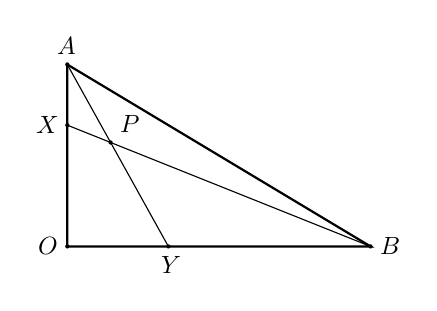
\begin{tikzpicture}[scale=0.55,every node/.style={font=\small}]
\coordinate(O)at(0,0);\coordinate(A)at(0,4.2);\coordinate(B)at(7,0);
\coordinate(X)at(0,2.8);\coordinate(Y)at(2.3333,0);\coordinate(P)at(1,2.4);
\draw[thick](O)--(A)--(B)--cycle;\draw(A)--(Y);\draw(B)--(X);
\foreach \n in {O,A,B,X,Y,P}{\fill (\n) circle(1.4pt);}
\node[left]at(O){$O$};\node[above]at(A){$A$};\node[right]at(B){$B$};
\node[left]at(X){$X$};\node[below]at(Y){$Y$};\node[above right]at(P){$P$};
\end{tikzpicture}\end{center}
\begin{enumerate}[label=(\alph*)]
\item By expressing $\vv{OP}$ in two ways using the ratio theorem, find $\vv{OP}$ in terms of $\mathbf a$ and $\mathbf b$. \mk{6}
\item Find $AP:PY$ and $BP:PX$. \mk{2}
\item The point $Z$ divides $AB$ internally with $AZ:ZB=1:4$. Show that $O,P,Z$ are collinear and find $OP:PZ$. \mk{2}
\end{enumerate}
\clearpage
\q{7}{6}A solid house consists of a cuboid $OBCDEFGH$ and a triangular prism roof $EFPHGQ$, as shown. The base $OBCD$ is horizontal. The vertices $E$, $F$, $G$ and $H$ are directly above $O$, $B$, $C$ and $D$ respectively.

The front-left corner $O$ is the origin. The positive $\mathbf i$, $\mathbf j$ and $\mathbf k$ directions are along $OB$, $OD$ and $OE$ respectively, and each unit represents $1$ metre. It is given that $OB=6\,\mathrm m$, $OD=4\,\mathrm m$ and $OE=3\,\mathrm m$.

The ridge $PQ$ is parallel to $OD$. The front gable $EFP$ and back gable $HGQ$ are congruent isosceles triangles, with $P$ vertically above the midpoint of $EF$ and $Q$ vertically above the midpoint of $HG$. Each sloping roof face makes an angle $\alpha$ with the horizontal, where $\tan\alpha=\frac23$; the vertical roof rise is $2\,\mathrm m$.
\begin{center}
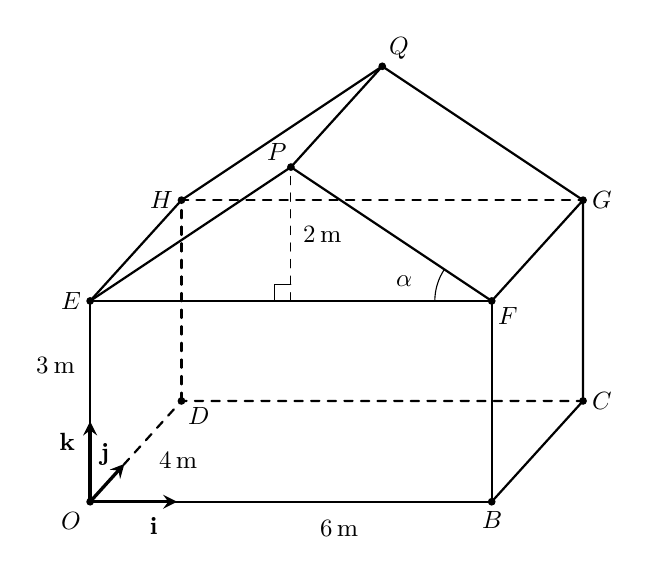
\begin{tikzpicture}[
  x={(0.85cm,0cm)},
  y={(0.29cm,0.32cm)},
  z={(0cm,0.85cm)},
  line join=round, line cap=round, >=stealth,
  every node/.style={font=\small}
]
\coordinate(O)at(0,0,0);
\coordinate(B)at(6,0,0);
\coordinate(C)at(6,4,0);
\coordinate(D)at(0,4,0);
\coordinate(E)at(0,0,3);
\coordinate(F)at(6,0,3);
\coordinate(G)at(6,4,3);
\coordinate(H)at(0,4,3);
\coordinate(P)at(3,0,5);
\coordinate(Q)at(3,4,5);
\coordinate(M)at(3,0,3);
% hidden edges
\draw[dashed,thick](O)--(D)--(C);
\draw[dashed,thick](D)--(H)--(G);
% visible edges
\draw[thick](O)--(B)--(F)--(E)--cycle;
\draw[thick](B)--(C)--(G)--(F);
\draw[thick](E)--(P)--(F);
\draw[thick](P)--(Q)--(G);
\draw[thick](E)--(H)--(Q);
% roof rise and angle
\draw[dashed](M)--(P);
\draw ($(M)+(-0.25,0,0)$)--++(0,0,0.25)--++(0.25,0,0);
\node[right=1pt] at ($(M)!0.5!(P)$) {$2\,\mathrm{m}$};
\draw ($(F)+(-0.85,0,0)$) arc[start angle=180, end angle=146.31, radius=0.85*0.85cm];
\node at ($(F)+(-1.30,0,0.30)$) {$\alpha$};
% lengths
\node[below=3pt] at ($(O)!0.62!(B)$) {$6\,\mathrm{m}$};
\node[below right=1pt] at ($(O)!0.62!(D)$) {$4\,\mathrm{m}$};
\node[left=2pt] at ($(O)!0.68!(E)$) {$3\,\mathrm{m}$};
% axes
\draw[->,very thick](O)--(1.3,0,0);
\node[below=2pt] at (0.95,0,0) {$\mathbf{i}$};
\draw[->,very thick](O)--(0,1.5,0);
\node[above left=-1pt] at (0,1.15,0) {$\mathbf{j}$};
\draw[->,very thick](O)--(0,0,1.2);
\node[left=2pt] at (0,0,0.9) {$\mathbf{k}$};
\foreach \n in {O,B,C,D,E,F,G,H,P,Q} {\fill(\n) circle (1.4pt);}
\node[below left] at (O) {$O$};
\node[below] at (B) {$B$};
\node[right] at (C) {$C$};
\node[below right=-1pt] at (D) {$D$};
\node[left] at (E) {$E$};
\node[below right=-1pt] at (F) {$F$};
\node[right] at (G) {$G$};
\node[left] at (H) {$H$};
\node[above left=-1pt] at (P) {$P$};
\node[above right=-1pt] at (Q) {$Q$};
\end{tikzpicture}\par
{\small All lengths are in metres. The diagram is not drawn to scale.}
\end{center}Find the coordinates of all the vertices of the house $(O,B,C,D,\ldots)$.
\q{8}{3}The diagram shows a container with a horizontal rectangular base $OABC$, where $OA=16\,\mathrm{cm}$ and $AB=11\,\mathrm{cm}$. The top of the container $DEFG$ is also a horizontal rectangle, where $DE=10\,\mathrm{cm}$ and $EF=5\,\mathrm{cm}$. The four sloping faces (for example $OAED$) of the container, each a trapezium, are inclined at the same angle to the horizontal, and the vertical distance between the base and the top is $6\,\mathrm{cm}$.

The point $O$ is taken as the origin $(0,0,0)$, and perpendicular unit vectors $\mathbf i$, $\mathbf j$, $\mathbf k$ are such that $\mathbf i$ is parallel to $OA$, $\mathbf j$ is parallel to $OC$, and $\mathbf k$ is vertical.
\begin{center}
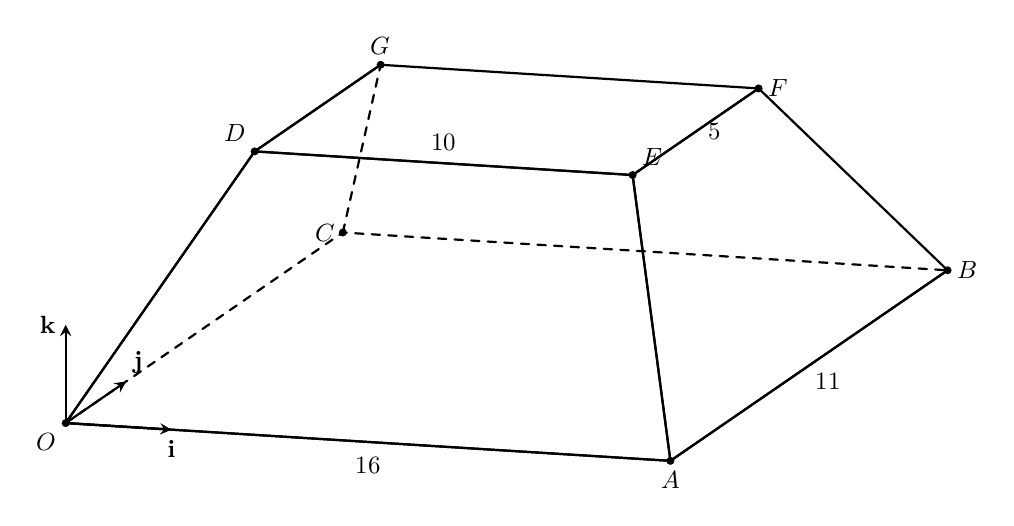
\begin{tikzpicture}[
  x={(0.48cm,-0.03cm)},
  y={(0.32cm,0.22cm)},
  z={(0cm,0.48cm)},
  line join=round, line cap=round, >=stealth,
  every node/.style={font=\bfseries\small}
]
\coordinate(O)at(0,0,0);
\coordinate(A)at(16,0,0);
\coordinate(B)at(16,11,0);
\coordinate(C)at(0,11,0);
\coordinate(D)at(3,3,6);
\coordinate(E)at(13,3,6);
\coordinate(F)at(13,8,6);
\coordinate(G)at(3,8,6);
\draw[dashed,thick](O)--(C)--(B);
\draw[dashed,thick](C)--(G);
\draw[thick](O)--(A)--(B);
\draw[thick](O)--(A)--(E)--(D)--cycle;
\draw[thick](A)--(B)--(F)--(E)--cycle;
\draw[thick](D)--(E)--(F)--(G)--cycle;
\draw[thick](O)--(D);
\draw[thick](G)--(D);
\draw[->,thick](O)--(2.8,0,0) node[below] {$\mathbf{i}$};
\draw[->,thick](O)--(0,2.4,0) node[above right=-1pt] {$\mathbf{j}$};
\draw[->,thick](O)--(0,0,2.6) node[left] {$\mathbf{k}$};
\foreach \n in {O,A,B,C,D,E,F,G} {\fill(\n) circle (1.45pt);}
\node[below left] at (O) {$O$};
\node[below] at (A) {$A$};
\node[right] at (B) {$B$};
\node[left] at (C) {$C$};
\node[above left] at (D) {$D$};
\node[above right] at (E) {$E$};
\node[right] at (F) {$F$};
\node[above] at (G) {$G$};
\node[below=2pt] at ($(O)!0.5!(A)$) {$16$};
\node[below right=-1pt] at ($(A)!0.5!(B)$) {$11$};
\node[above=1pt] at ($(D)!0.5!(E)$) {$10$};
\node[right=1pt] at ($(E)!0.5!(F)$) {$5$};
\end{tikzpicture}\par
{\small All lengths are in centimetres. The diagram is not drawn to scale.}
\end{center}Find the coordinates of $D$.
\medskip\begin{center}\textbf{END OF HOMEWORK}\end{center}\end{document}